\newpage

\section{IPSec VPN Configuration}

This section details the configuration of the IPSec-based VPN connection using strongSwan as the client software. The IPSec implementation provides network-layer security with encryption and authentication, establishing a secure tunnel between the client container and the SoftEther VPN server.

\subsection{strongSwan Client Setup}

The strongSwan software was installed during the initial container configuration as part of Section 4. To verify the installation and ensure all components are available:

\begin{lstlisting}[language=bash]
# Verify strongSwan installation
apt list --installed | grep strongswan

# Check available strongSwan tools
which ipsec

\end{lstlisting}

\subsection{IPSec Configuration Files}

strongSwan uses two primary configuration files: \texttt{ipsec.conf} for connection parameters and \texttt{ipsec.secrets} for authentication credentials.

\subsubsection{ipsec.conf Analysis}

The \texttt{ipsec.conf} file defines the IPSec connection parameters, including encryption algorithms, authentication methods, and tunnel endpoints.

\begin{lstlisting}[language=bash]
# /etc/ipsec.conf
config setup
    charondebug="ike 2, knl 2, cfg 2"   # Debugging levels
    uniqueids=yes                       # Ensure unique IDs

conn softether
    # Local settings
    left=%any                          # Accept any local IP
    leftsubnet=10.0.2.0/24             # Client subnet to encrypt
    leftid=@client                     # Unique client identifier
    
    # Remote settings  
    right=203.0.113.1                  # Server public IP
    rightid=10.0.1.2                   # Server's actual IP
    rightsubnet=0.0.0.0/0              # All traffic via VPN
    
    # NAT-Traversal
    forceencaps=yes                     # Force UDP encapsulation
    
    # Phase 1 (IKEv1)
    keyexchange=ikev1                   # Use IKEv1 protocol
    ike=aes256-sha1-modp2048!           # IKE encryption
    esp=aes128-sha1-modp1024!           # ESP encryption
    aggressive=no                       # Use main mode
    
    # Authentication
    leftauth=psk                        # Pwd authentication
    rightauth=psk                       # Server uses PSK too
    
    # Dead Peer Detection
    dpdaction=restart                   # Restart on peer failure
    dpddelay=30s                        # DPD check interval
    dpdtimeout=120s                     # DPD timeout
    
    auto=start                          # Auto-start connection
\end{lstlisting}

\noindent
\textbf{Configuration Parameter Explanation:}

\begin{itemize}
    \item \textbf{Connection Identity:} \texttt{left/right} parameters define local and remote endpoints
    \item \textbf{Subnet Configuration:} \texttt{leftsubnet} specifies which traffic should be encrypted
    \item \textbf{NAT Traversal:} \texttt{forceencaps=yes} ensures IPSec works through NAT devices
    \item \textbf{Algorithm Selection:} Encryption with AES-256 for IKE and AES-128 for ESP, also here the usage of a weak hash function (SHA1) is only for lab purposes.
    \item \textbf{Authentication:} Pre-shared key (PSK) method matching server configuration
    \item \textbf{Dead Peer Detection:} Automatic tunnel recovery on connection failure
\end{itemize}

\subsubsection{ipsec.secrets Configuration}

The \texttt{ipsec.secrets} file contains authentication credentials, specifically the pre-shared key that must match the server configuration.

\begin{lstlisting}[language=bash]
# /etc/ipsec.secrets
# Format: local_id remote_id : PSK "shared_secret"

%any 203.0.113.1 : PSK "ciao"
\end{lstlisting}

\textbf{Authentication Details:}

\begin{itemize}
    \item \textbf{Local ID:} \texttt{\%any} accepts any local IP address
    \item \textbf{Remote ID:} \texttt{203.0.113.1} specifies the SoftEther server's public IP
    \item \textbf{Authentication Method:} PSK (Pre-Shared Key)
    \item \textbf{Shared Secret:} "ciao" - must match the server's IPSec\_Secret configuration
\end{itemize}

\noindent
\textbf{Important Security Note:} In production environments, pre-shared keys should be significantly more complex and randomly generated. The simple "ciao" key is used here for laboratory demonstration purposes only.

\subsection{Connection Establishment}

The IPSec tunnel establishment process involves multiple phases, including IKE negotiation and ESP Security Association creation.

\subsubsection{Manual Connection Initiation}

To establish the IPSec connection manually:

\begin{lstlisting}[language=bash]
# Restart strongSwan to reload configuration
ipsec restart

# Initiate the VPN connection
ipsec up softether

# Verify connection status
ipsec status

# Check established Security Associations
ipsec statusall
\end{lstlisting}

\subsubsection{Connection Verification}

Successful IPSec tunnel establishment can be verified through multiple methods:

\begin{lstlisting}[language=bash]
# Test connectivity through tunnel
ping 192.168.30.1  # SoftEther SecureNAT gateway

# Check routing table for VPN routes
ip route show

\end{lstlisting}

\subsubsection{Debug and Troubleshooting}

For troubleshooting connection issues, strongSwan provides comprehensive debugging:

\begin{lstlisting}[language=bash]
# Start strongSwan with full debugging
ipsec start --nofork --debug-all

# Verify network connectivity to server
ping 203.0.113.1

\end{lstlisting}

\subsection{Traffic Analysis}

Understanding how IPSec encapsulates and processes network traffic is crucial for verification and troubleshooting.

\subsubsection{Wireshark Packet Analysis}

To observe IPSec traffic in detail, it is highly recommended to open a Wireshark instance on one of the network cables connecting the client and server infrastructure. This allows real-time analysis of the VPN establishment and data transmission phases.

\noindent
\\
\textbf{IPSec Tunnel Establishment Phase:}

\noindent
During the initial IPSec connection setup, Wireshark will capture ISAKMP (Internet Security Association and Key Management Protocol) packets. You can start the Wireshark capture instance by right clicking on a wire in GNS3, and then selecting "Start Capture".

\begin{figure}[H]
\centering
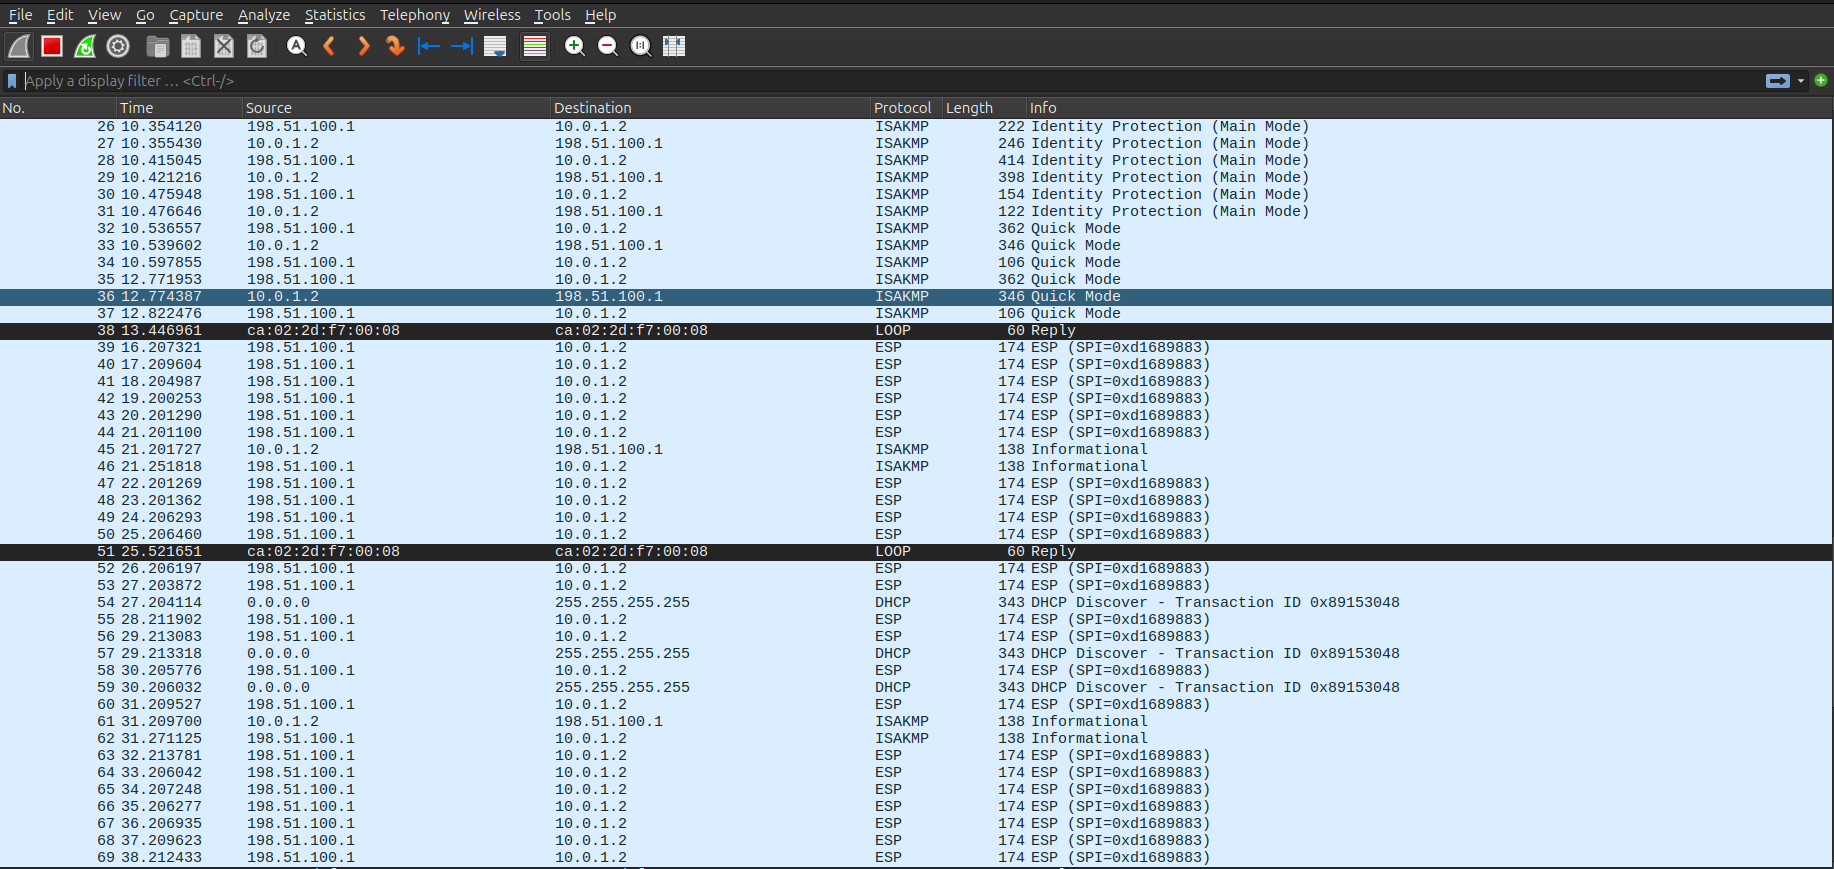
\includegraphics[width=\textwidth]{../resources/Images/IPsec_Packets.png}
\caption{IPSec VPN Traffic Analysis - ISAKMP and ESP Protocol Exchange}
\label{fig:ipsec_packets}
\end{figure}

Figure \ref{fig:ipsec_packets} demonstrates a comprehensive IPSec VPN session captured with Wireshark, showing the complete lifecycle of an IPSec tunnel establishment and data transmission. The capture reveals several distinct phases:

\noindent

\textbf{ISAKMP Phase 1 (Main Mode):} The initial packets (frames 26-31) show the ISAKMP Main Mode negotiation on UDP port 500, where the VPN endpoints establish the first Security Association (SA) for protecting subsequent key exchange traffic. This phase includes:
\begin{itemize}
    \item Identity Protection exchange for secure peer authentication
    \item Negotiation of encryption and authentication algorithms
    \item Diffie-Hellman key exchange for establishing shared secrets
\end{itemize}

\noindent
\\
\textbf{ISAKMP Phase 2 (Quick Mode):} Following the main mode, Quick Mode packets establish the Security Associations for actual data protection, negotiating the parameters for ESP (Encapsulating Security Payload) tunnels.

\noindent
\\
\textbf{ESP Data Transmission:} The latter portion of the capture shows ESP packets carrying encrypted user data. These packets demonstrate the IPSec tunnel in operation, where all original IP traffic is encapsulated within ESP headers and encrypted according to the negotiated algorithms.

\noindent
\\
\textbf{Active Tunnel Communication Phase:}

\noindent
Once the IPSec tunnel is established and active communication begins, the packet capture will show ESP (Encapsulating Security Payload) packets:

\begin{lstlisting}[language=bash]
# Filter for ESP traffic during active communication

# Test communication to generate ESP traffic
ping 192.168.30.1  # From client to SoftEther SecureNAT
\end{lstlisting}

\noindent
During active communication, you will observe:
\begin{itemize}
    \item \textbf{ESP packets:} Encrypted data transmission with visible ESP headers
    \item \textbf{Encrypted payload:} Data content protected by IPSec encryption
    \item \textbf{Tunnel endpoints:} Source and destination IPs showing the VPN gateway addresses
\end{itemize}

